\chapter{Evaluation}
In a sense, evaluating this project should not be necessary: it is \emph{verified}, so the reasoning (if not the definitions) within it cannot be doubted without also doubting the correctness of Isabelle itself.
However, there are other metrics to the project's success other than its relative truth:
\begin{itemize}
\item
Practical examples: while the implementation is theoretically correct with respect to a set of definitions, these definitions must correspond to an intuitive understanding of what the implementation should do.
Therefore, manually-written tests should check the expected properties of the calculus to avoid vacuous or controversial definitions.
\item
Performance: extracted algorithms should perform well, at least asymptotically.
It is difficult to argue this directly in a proof assistant, so it is easier to produce empirical data and show that statistically the algorithm works as expected.
\item
Comparison to other work: of course, there is existing academic work in this general area, and comparisons must be drawn to highlight successes and failures in my approach.
The choice of representation especially in the project is somewhat unusual, and comes with advantages and disadvantages compared to other approaches.
\end{itemize}

The majority of the practical evaluation was directed at the extracted type inference algorithm, but there is also some testing of freshened variables and the representation of the calculus itself.

\section{Framework for Evaluation}
Isabelle supports four programming languages in its code-extraction machinery: Standard ML, OCaml, Haskell, and Scala\cite{codegen-reference}.
Haskell was the chosen language for evaluating the type inference algorithm: it offered better library and runtime support for testing and benchmarking than Standard ML and OCaml, but remained closer to the algorithm expressed in Isabelle than Scala (which has a more complex type system).
To build and evaluate the extracted code, I used Stack\cite{stack}, a tool for Haskell that provides sandboxing, compiler and package isolation, build systems, and support for running tests and benchmarks, in combination with GHC\cite{GHC}, the \emph{de facto} Haskell compiler.

Isabelle's code extraction mechanism immediately produced correct code that resembled the formalisation very well without further tweaking, but there were several problems that needed to be fixed without touching (and thereby invalidating) the extracted code.
I added a new module \emph{Utils} to the extracted code which provided some utilities for testing and benchmarking and fixed the problems:
\begin{itemize}
\item
The extracted code initially wouldn't compile, as it produced invalid Haskell type signatures that are neither Haskell '98 nor Haskell 2010.
The type signatures added explicit universal quantification to type variables, where usually the compiler would infer that all type variables were implicitly universally quantified.
For example, the polymorphic identity function in standard Haskell
\begin{minted}{Haskell}
id :: a -> a
id x = x
\end{minted}
became
\begin{minted}{Haskell}
id :: forall a. a -> a
id x = x
\end{minted}
However, this could be made to build using the \emph{ExplicitForAll} GHC extension, which allows this syntax (albeit only to instrument more useful extensions).
\item
Extracted code often implemented its own version of standard Haskell typeclasses, (such as that for partial orders), implemented but did not instantiate a typeclass, or did not implement/export useful functions (such as serialisation functions).
In all cases typeclass instances could be provided easily:
standard Haskell typeclasses can be implemented in terms of the custom typeclasses,
\begin{minted}{Haskell}
instance Ord Nat where
  (<=) = Orderings.less_eq
\end{minted}
instances can be provided \emph{ex post facto} in Haskell,
\begin{minted}{Haskell}
instance Eq Nat where
  (==) = equal_nat
\end{minted}
and trivial typeclass instances can be implemented manually, or, more efficiently, using the \emph{StandaloneDeriving} extension
\begin{minted}{Haskell}
deriving instance Show Nat
deriving instance Read Nat
\end{minted}
\item
In a similar vein, despite extracting both a typeclass for fresh variables and an implementation of the typeclass for natural numbers, the code extraction failed to join the two, so
\begin{minted}{Haskell}
instance Fresh Nat where
  fresh_in = fresh_in_nat
\end{minted}
had to be added manually to use the freshness implementation.
\end{itemize}
\section{Practical Examples and Property Testing}
A common method of testing software is unit testing, in which code is subjected to single pass/fail test units.
This works well for most cases, but the mathematical nature of the domain means that lots of test cases ought to be universally quantified over their inputs, rather than a fixed constant as in unit testing.
Property testing, on the other hand, generates random test data and checks a property holds for all of them.
This technique is more well-suited to the problem: it approximates universal quantification, and the random inputs find edge-cases quickly.

To implement property testing, I used HSpec\cite{hspec}, a library for structuring Haskell tests, combined with QuickCheck\cite{quickcheck}, a library for property testing.
A test program using these libraries looks like figure \ref{fig:example-test}.

%TC:ignore
\begin{figure}
\begin{minted}{Haskell}
main :: IO ()
main = hspec $ do
  describe "unit inference" $ do
    it "infers unit values to have unit type" $ do
      property $
        forAll contexts $ \c ->
        infer' c PUnit `shouldBe` pure TUnit
\end{minted}
\caption{an example test program: this asserts that, for all typing contexts \(c\), the inferred type of a unit value is the unit type}
\label{fig:example-test}
\end{figure}
%TC:endignore

One problem with property testing \`a-la-QuickCheck is that random generators for all tested types have to be written.
QuickCheck provides generators for all basic types, and some derived ones via a typeclass mechanism (e.g. if you have generators for types \(t_1\) and \(t_2\), you also have a generator for \(t_1 \times t_2\)), but any new types introduced have to have custom generators written.
I wrote generators for natural numbers, types, typing contexts, and pre-terms, and also for ill-typed and well-typed terms.

With these generators, I then wrote tests that asserted, in the context of various categories, the following propositions --- note the similarity in structure to the inductive typing judgements.
Write \(\infer(\Gamma, M)\) for the result of running the inference algorithm with context \(\Gamma\) on term \(M\), and use \(\bot\) to indicate a type error.
Consider all free variables universally quantified (i.e. randomly-generated in the test).
\begin{itemize}
\item fresh variables:
\begin{itemize}
\item a fresh \(x\) generated with respect to \(S\) has the property \(x \notin S\)
\end{itemize}
\item unit inference:
\begin{itemize}
\item \(\infer(\Gamma, \unit) = 0\)
\end{itemize}
\item variable inference:
\begin{itemize}
\item any variable \(x\) satisfies \(\infer(\emptyset, x) = \bot\)
\item if \(x\) is fresh in the domain of \(\Gamma\), \(\infer(\emptyset, x) = \bot\)
\item if there is a \(\tau\) such that \(\Gamma(x) = \tau\), then \(\infer(\emptyset, x) = \tau\)
\end{itemize}
\item \(\lambda\)-inference:
\begin{itemize}
\item if \(\infer(\Gamma\{x \mapsto \tau\}, M) = \bot\), then \(\infer(\Gamma, \lambda (x : \tau). M) = \bot\)
\item for all variables \(x\), \(y\), \(x \neq y\) implies that \(y\) is not bound in the expression \(\lambda (x : \tau). y\)
\item if \(\infer(\Gamma\{x \mapsto \tau\}, M) = \sigma\), then \(\infer(\Gamma,\lambda (x : \tau). M) = \tau \to \sigma\)
\end{itemize}
\item application inference:
\begin{itemize}
\item if \(\infer(\Gamma, M) = \bot\), \(\infer(\Gamma, (M\ N)) = \bot\)
\item also, if \(\infer(\Gamma, N) = \bot\), \(\infer(\Gamma, (M\ N)) = \bot\)
\item if \(\infer(\Gamma, M) = T\) and \(T\) is not of the form \(\tau \to \sigma\), then \(\infer(\Gamma, (M\ N)) = \bot\)
\item if \(T\) \emph{is} of the form \(\tau \to \sigma\), but \(\infer(\Gamma, N) \neq \tau\), then \(\infer(\Gamma, (M\ N)) = \bot\)
\item finally, if \(\infer(\Gamma, N) = \tau\), then \(\infer(\Gamma, (M\ N)) = \sigma\)
\end{itemize}
\item pair inference:
\begin{itemize}
\item if \(\infer(\Gamma, M) = \bot\), then \(\infer(\Gamma, (M, N)) = \bot\)
\item also, if \(\infer(\Gamma, N) = \bot\), then \(\infer(\Gamma, (M, N)) = \bot\)
\item if \(\infer(\Gamma, M) = \tau_1\) and \(\infer(\Gamma, N) = \tau_2\), then \(\infer(\Gamma, (M, N)) = \tau_1 \times \tau_2\)
\end{itemize}
\item projection inference:
\begin{itemize}
\item if \(\infer(\Gamma, M) = \bot\), then \(\infer(\Gamma, \pi_1(M)) = \bot\) and \(\infer(\Gamma, \pi_2(M)) = \bot\)
\item if \(\infer(\Gamma, M) = T\), but \(T\) is not of the form \(\tau_1 \times \tau_2\), then \(\infer(\Gamma, \pi_1(M)) = \bot\) and \(\infer(\Gamma, \pi_2(M)) = \bot\)
\item if \(T\) is of the form \(\tau_1 \times \tau_2\), then \(\infer(\Gamma, \pi_1(M)) = \tau_1\) and \(\infer(\Gamma, \pi_2(M)) = \tau_2\)
\end{itemize}
\item testing assumptions
\begin{itemize}
\item if a term \(M\) is generated from the ill-typed pool, \(\infer(\Gamma, M) = \bot\)
\item on the other hand, if \(M\) is generated from the well-typed pool, \(\infer(\Gamma, M) = \tau\) for some \(\tau\)
\end{itemize}
\end{itemize}

All tests pass, producing output similar to that shown in figure \ref{fig:tests-output}.
While property tests can never provide absolute confidence in the project (in this case the parameter space is infinite), they do produce empirical evidence to \emph{suggest} correctness.

\begin{figure}
\centering
\begin{minted}{text}
fresh variables
  fresh in a set
unit inference
  infers unit values to have unit type
inference of variables
  undefined in the empty context
  undefined if fresh in a context
  infers the correct type if in a context
inference of lambdas
  propagates type errors
  doesn't bind extraneous variables
  infers a correct type
inference of applications
  propagates type errors on the left
  propagates type errors on the right
  undefined for non-arrow application
  undefined for type mismatch
  infers correct type
inference of pairs
  propagates type errors on the left
  propagates type errors on the right
  infers correct type
inference of projection
  propagates type errors
  undefined for non-pair application
  infers correct type
testing assumptions
  ill-typed terms are ill-typed
  well-typed terms are well-typed

Finished in 48.3063 seconds
21 examples, 0 failures
\end{minted}
\caption{output from property testing}
\label{fig:tests-output}
\end{figure}

\section{Benchmarking and Performance}
Inputs to the type inference algorithm can be given a notion of size by counting the number of nodes in the syntax tree of the input.
For instance, the term \(\pi_1((\lambda (x : 0). (x, \unit))\ \unit)\) is shown in figure \ref{fig:example-tree} and has 7 syntactic nodes.
Formally, the size of a term \(M\), \(|M|\), can be given recursively by
\[
|M| =
\begin{cases}
1 & M = \unit\\
1 & M = x\\
1 + |M'| & M = \lambda (x : \tau). M'\\
1 + |A| + |B| & M = (A\ B)\\
1 + |A| + |B| & M = (A, B)\\
1 + |P| & M = \pi_1(P)\\
1 + |P| & M = \pi_2(P)\\
\end{cases}
\]

Given this, the formalised type inference algorithm can be seen (by induction) to have time complexity \(O(|M|)\) with respect to the input \(M\), assuming that finite map update/lookup operations are \(O(1)\).
However, it's difficult to see how to show this formally in Isabelle, and there is no reason to worry about performance until the code is extracted anyway --- at which point the code may have drastically different performance characteristics than the idealised formal specification.

Therefore, we are left to try and establish performance characteristics of the extracted code by the scientific method, rather than mathematically.

\begin{figure}
\centering
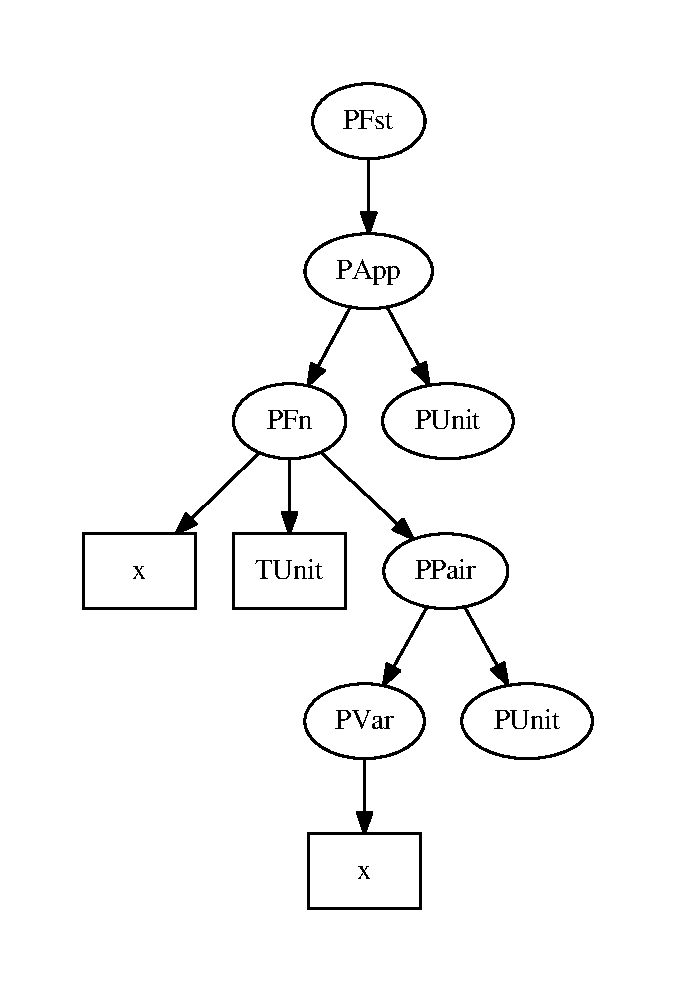
\includegraphics[height=4in]{chapters/evaluation/figures/example-tree.pdf}
\caption{an example syntax tree: syntactic nodes are shown by ellipses, with incidental data in boxes}
\label{fig:example-tree}
\end{figure}

\subsection{Experimental Method}
There is a problem in that asymptotic complexity cannot be determined by any performance measurements on finite inputs.
However, since type inference is only likely to be run on terms of a reasonable size, say, no more than \(10^5\), we can state that it has a certain asymptotic complexity within a given range of sizes.

The experimental approach, is as follows:
\begin{enumerate}
\item
Generate representative test data of several different orders of magnitude in the reasonable range.
\item
Benchmark the algorithm on each of these test inputs and record performance.
\item
Correlate (logarithmic) time-to-run against (logarithmic) input size to determine an asymptotic performance bound.
\end{enumerate}

\subsubsection{Generating Data}
Ideally the data generated would be (pseudo-) random, in order to prevent any patterns introduced in the test data from affecting the benchmark: the generators used to produce test data could then be repurposed to benchmark data.
Another constraint is that the expression must be well-typed in general, or the error propagating through will remove most of the processing from the benchmark.

Unfortunately, QuickCheck's random generation procedures turned out to be too slow to produce large randomised inputs efficiently.
Instead, I used deterministic algorithms to produce large inputs, according to a variety of patterns:
\begin{enumerate}
\item well-typed terms in a repeating pattern, using all datatype constructors
\item pairs, with each sub-term a pair
\item projection functions applied to pairs repeatedly
\item applications, with each sub-term of equal size
\item applications, with unbalanced sub-terms
\item function binders in a chain
\item a sequence of binders, followed by bound variables
\end{enumerate}
These are designed to test general performance on varied inputs, on specific inputs, and finally to stress the typing context operations.

I then used the patterns to generate data, sized from 1, increasing by a factor of 10 to 100,000, and wrote the data to file for reproducibility.

\subsubsection{Benchmarking}
Benchmarking algorithms on small inputs (``micro-benchmarking'') has the problem of jitter: outside factors such as cache effects, branch prediction and kernel scheduling can all cause the same algorithm with the same input to run at different rates.

Haskell's laziness also adds another problem --- since the parameter passed to the function is not strictly-evaluated, the first evaluation of the function can take significantly longer as in this case the input needs to be loaded from disk and parsed before being processed.

Both these problems were solved by using the Criterion micro-benchmarking library\cite{criterion}.
This solution deals with jitter by running the algorithm repeatedly and differing numbers of times to generate enough samples for a statistically significant result (generally an \(R^2\) value exceeding 0.99), and with laziness by evaluating the argument to a normal form first.

\subsection{Results}
Results were extremely positive for the \(O(|M|)\) hypothesis.
Figure \ref{fig:results-welltyped} shows a strong linear correlation for the general-performance dataset, while figure \ref{fig:results-combined} supports this further, showing that every sort of structure produces linear performance on the target range.
The high levels of correlation on every graph lend extra credit to the hypothesis of a linear-time algorithm.

\begin{figure}
\centering
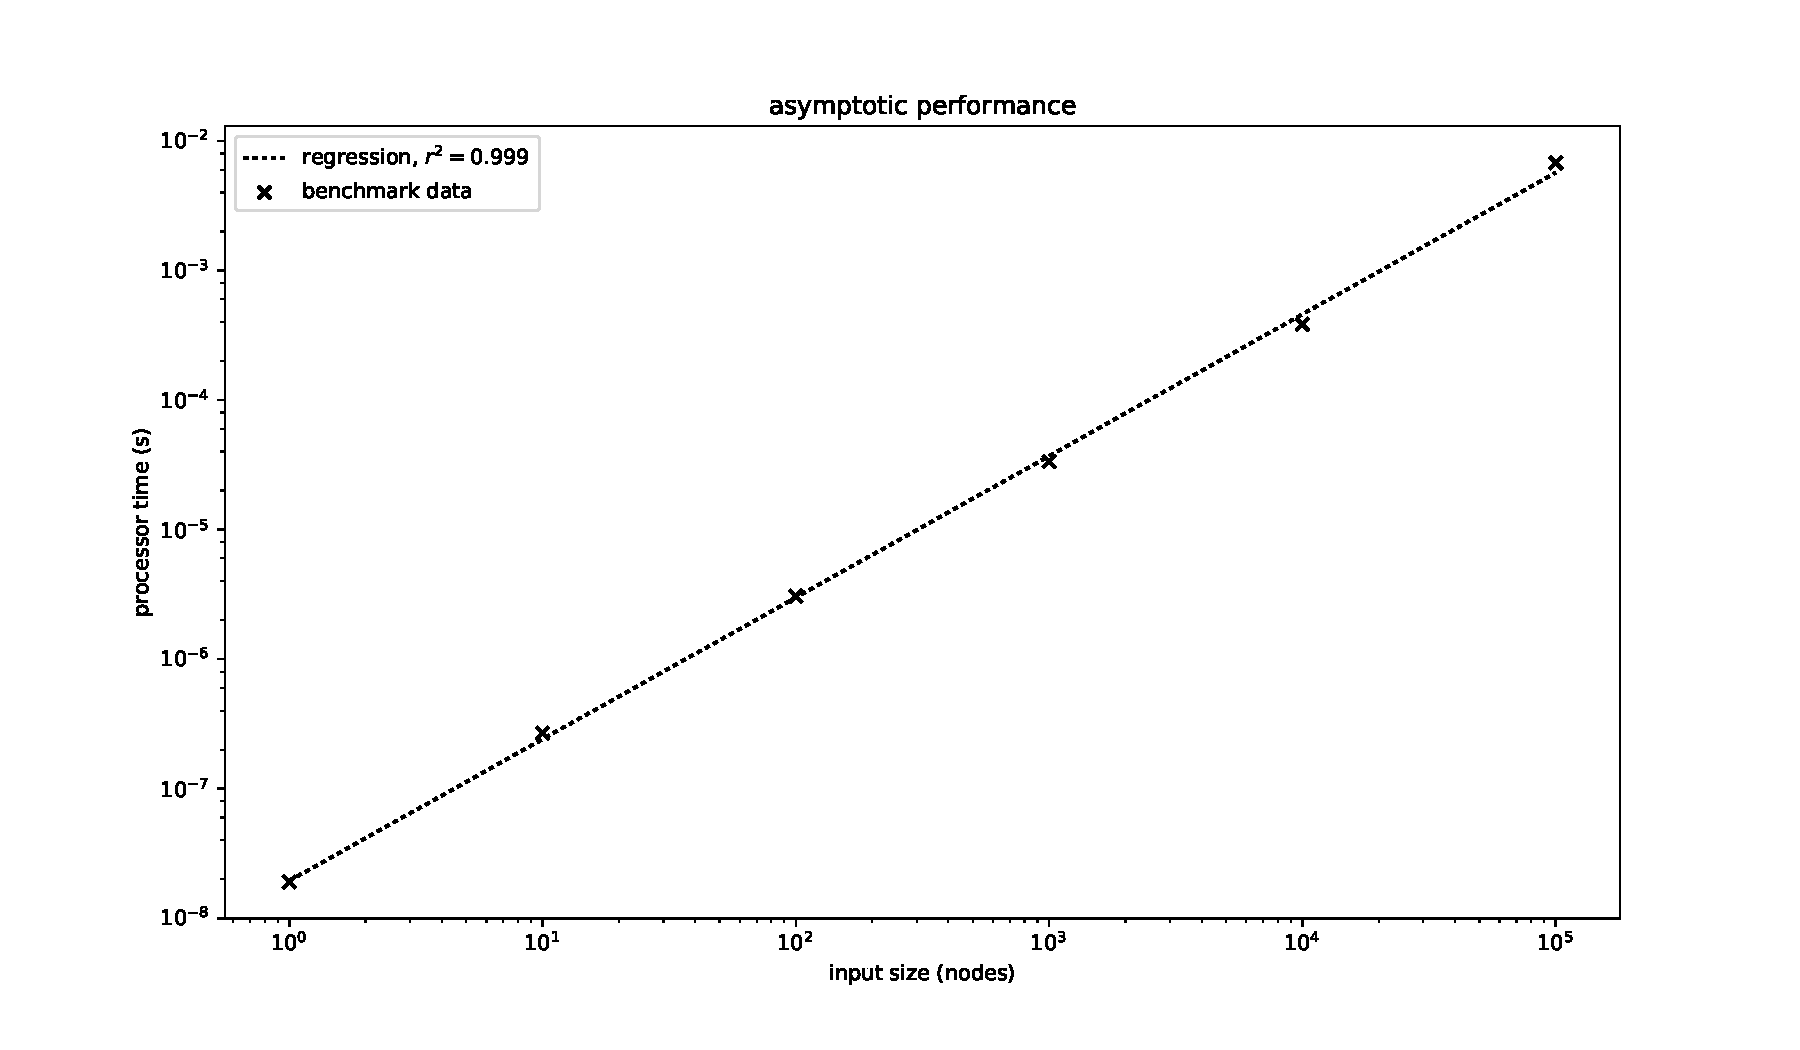
\includegraphics[width=\textwidth]{chapters/evaluation/plots/welltyped}
\caption{log-log plot of benchmark data size vs processor time, with a linear regression fitted}
\label{fig:results-welltyped}
\end{figure}

\begin{figure}
\centering
\begin{subfigure}{.49\textwidth}
 \centering
 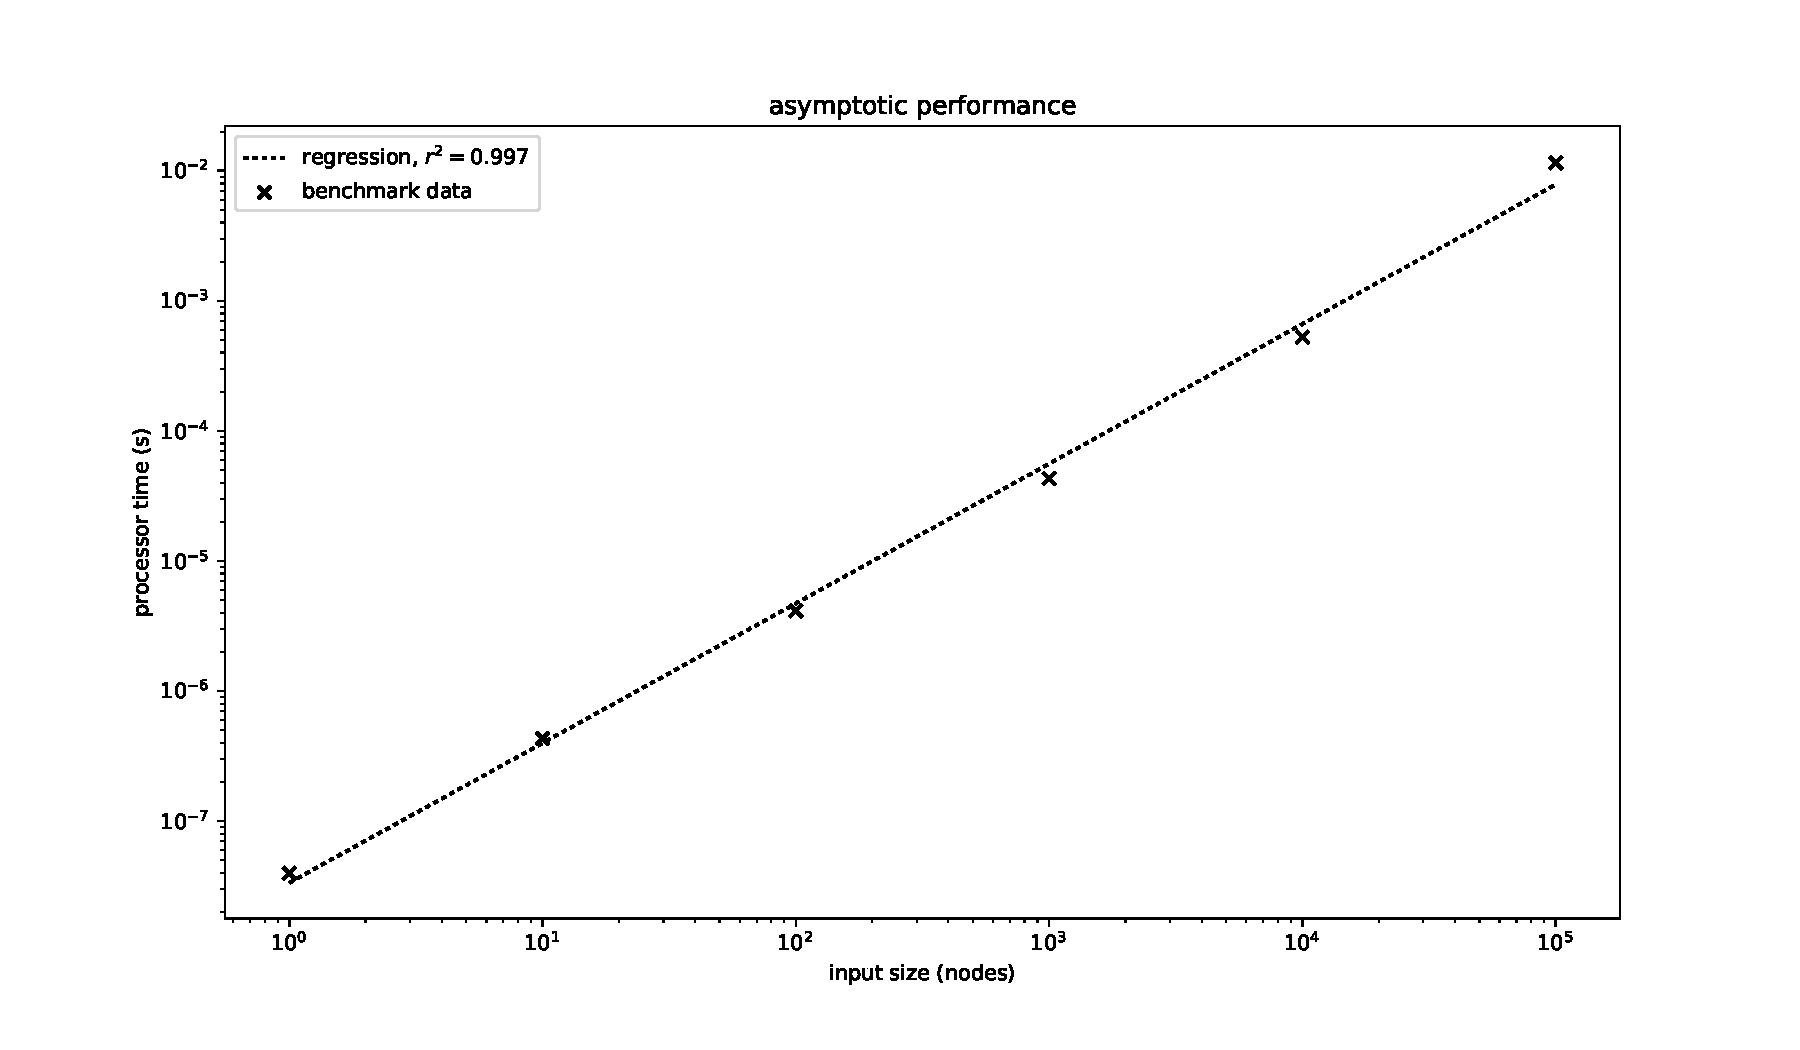
\includegraphics[width=\linewidth]{chapters/evaluation/plots/pair}
 \caption{pairs}
\end{subfigure}
\begin{subfigure}{.49\textwidth}
 \centering
 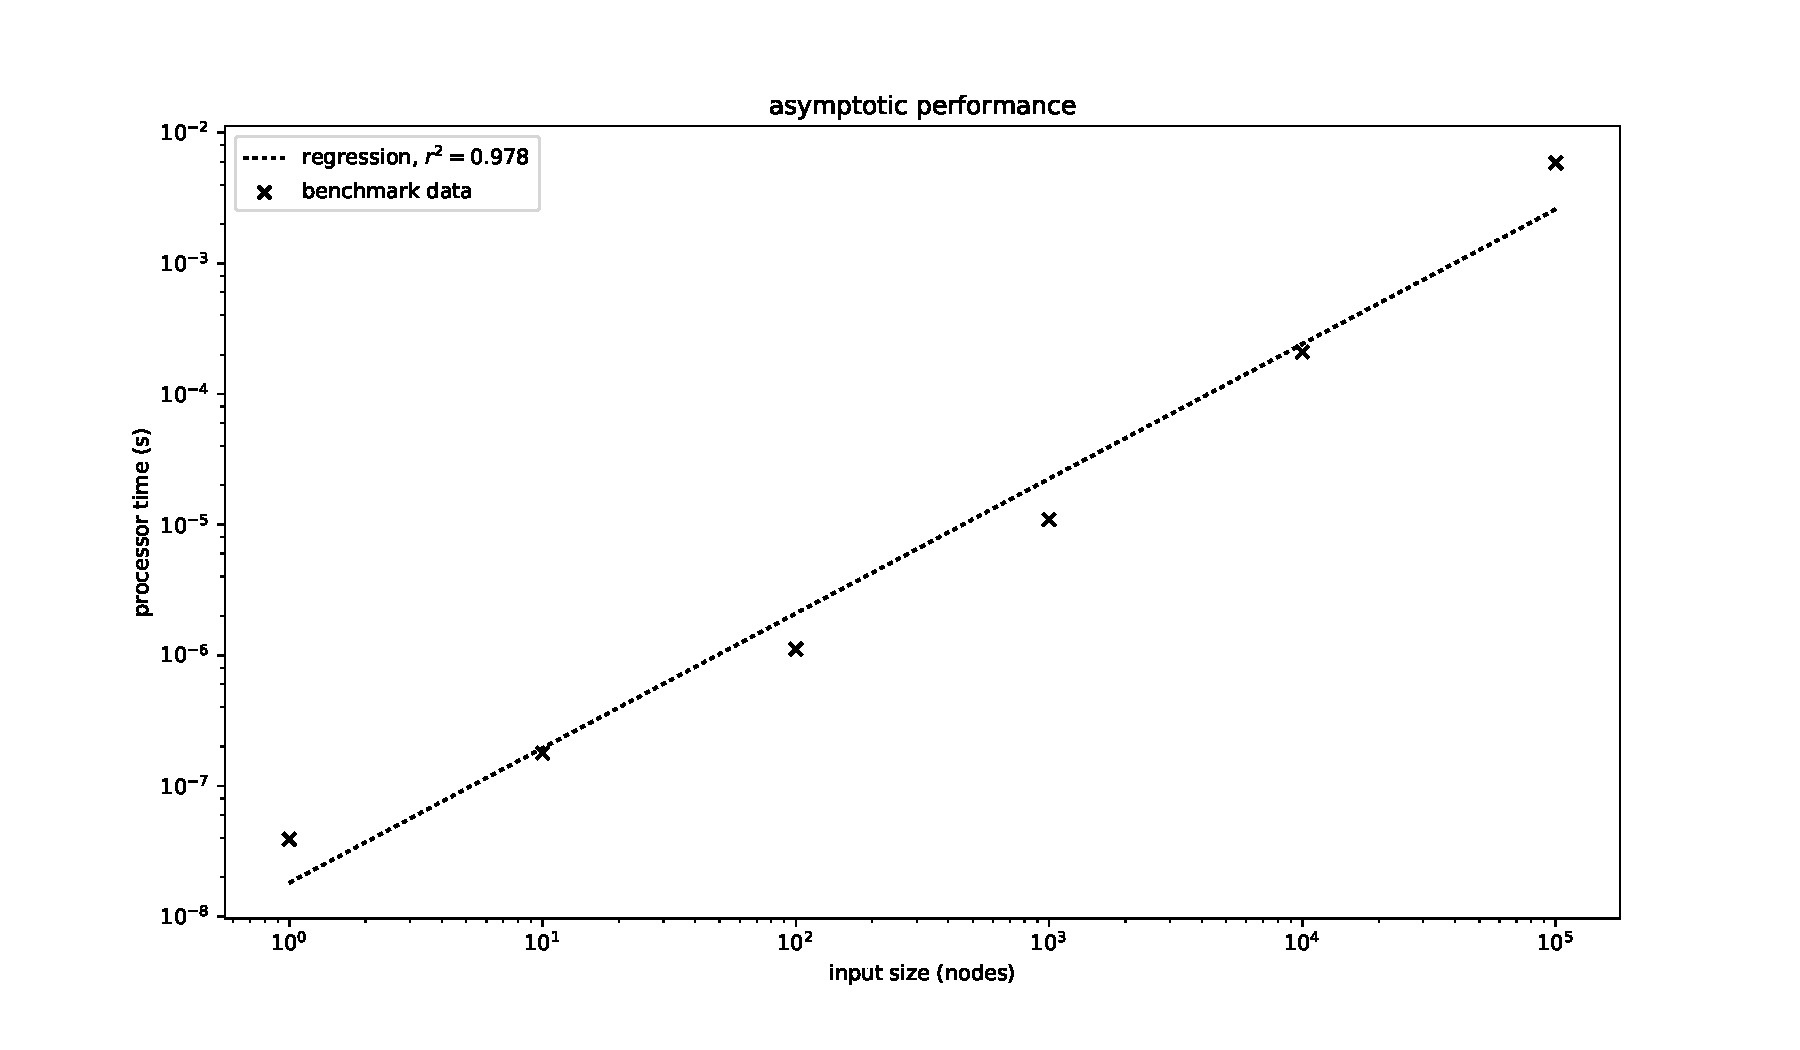
\includegraphics[width=\linewidth]{chapters/evaluation/plots/projections}
 \caption{projections}
\end{subfigure}
\begin{subfigure}{.49\textwidth}
 \centering
 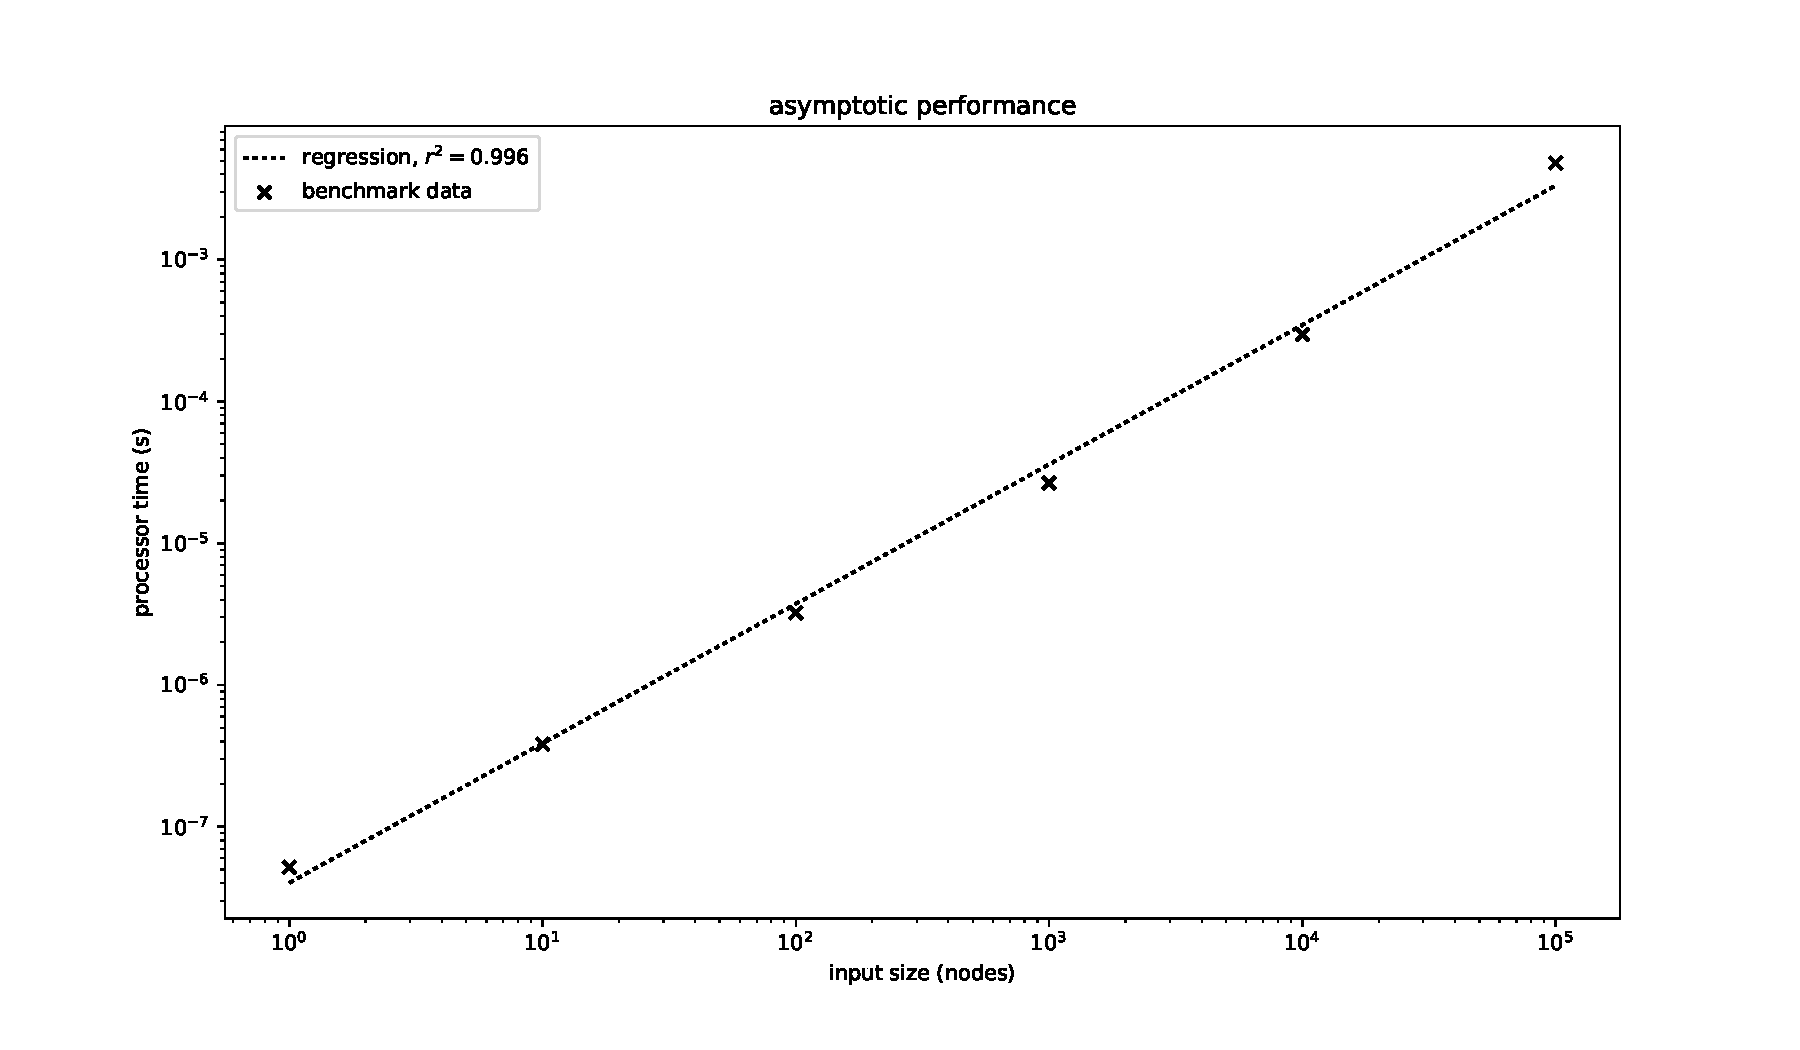
\includegraphics[width=\linewidth]{chapters/evaluation/plots/app}
 \caption{balanced applications}
\end{subfigure}
\begin{subfigure}{.49\textwidth}
 \centering
 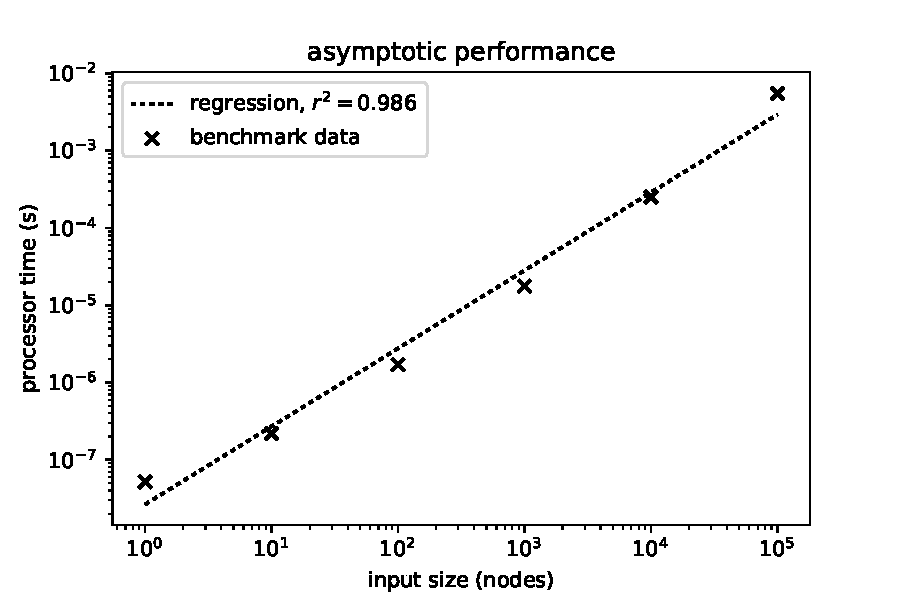
\includegraphics[width=\linewidth]{chapters/evaluation/plots/biased-app}
 \caption{applications, biased to one side}
\end{subfigure}
\begin{subfigure}{.49\textwidth}
 \centering
 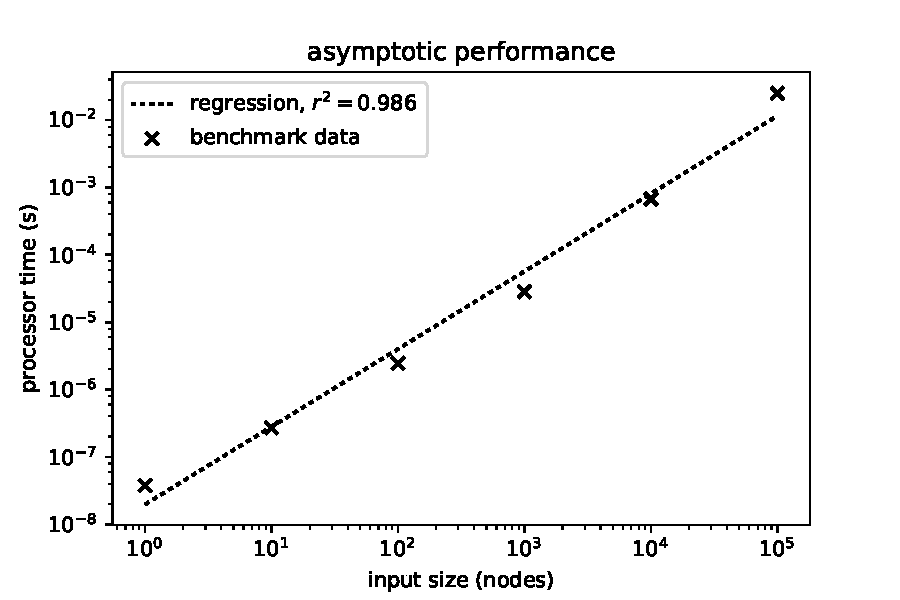
\includegraphics[width=\linewidth]{chapters/evaluation/plots/fn}
 \caption{chain of function binders}
\end{subfigure}
\begin{subfigure}{.49\textwidth}
 \centering
 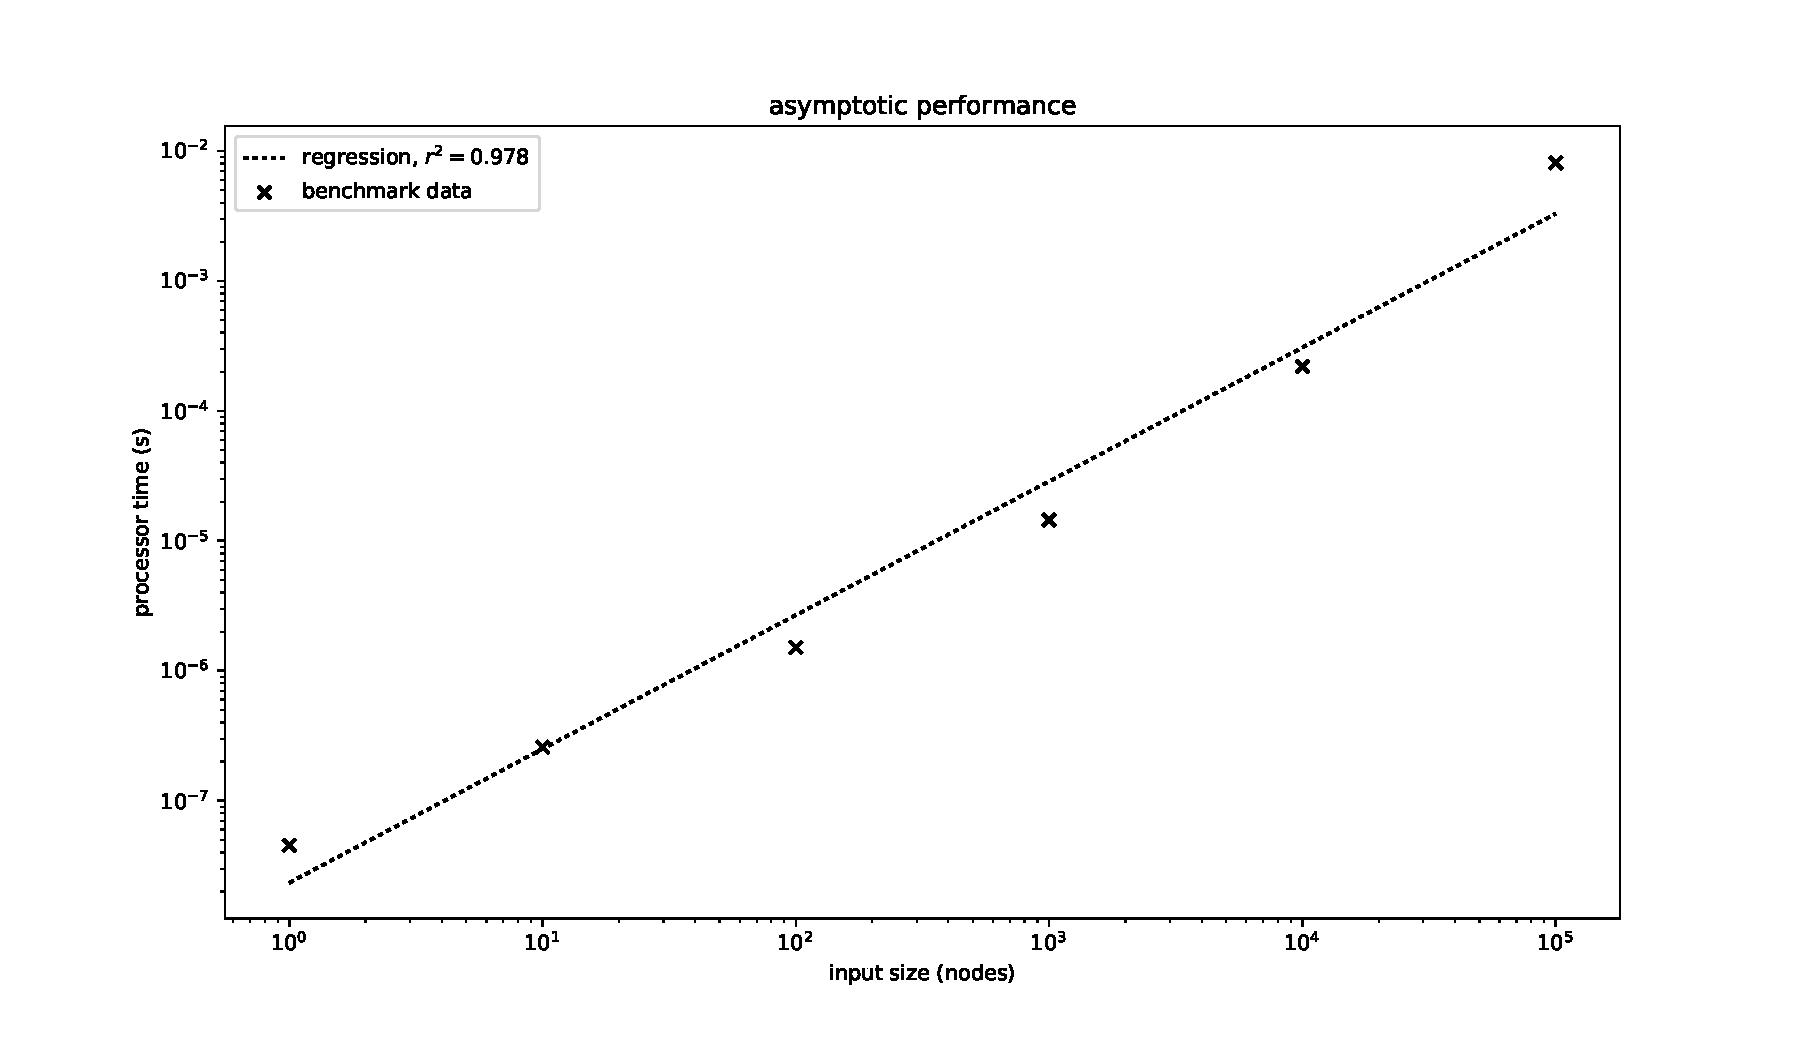
\includegraphics[width=\linewidth]{chapters/evaluation/plots/lookup}
 \caption{typing context stress}
\end{subfigure}
\caption{log-log plots (similar to figure \ref{fig:results-welltyped}), showing performance on specialised inputs}
\label{fig:results-combined}
\end{figure}

Of particular interest is the context stress-test: this was included as the extracted code uses a method of representing finite maps using closures that should be extremely inefficient.
It implements the lookup and update operations as follows:

\begin{minted}{Haskell}
type Context k a = k -> Maybe a

lookup :: Context k a -> k -> Maybe a
lookup c k = c k

update :: Eq k => Context k a -> k -> a -> Context k a
update c k a = \x -> if x == k then Just a else c x

empty :: Context k a
empty = \x -> Nothing
\end{minted}

In the case of the extracted inference algorithm, this implementation of map should result in quadratic slowdown when applied to binders followed by variable lookup, as the closure representing the finite map grows in size.
However, in the typing-context dataset, this does not appear to be the case: even profiling the executable does not show significant time spent in the closure, or in the equality implementation.

However, I would still expect a reasonable implementation with e.g. an ordered map to be more performant: figure \ref{fig:results-map} shows that a hand-implemented version using Haskell's \emph{containers} ordered-map implementation is still linear in the size of the input (as expected), but the implementation is considerably slower than the na\"ive version.

\begin{figure}
\begin{subfigure}{.49\textwidth}
 \centering
 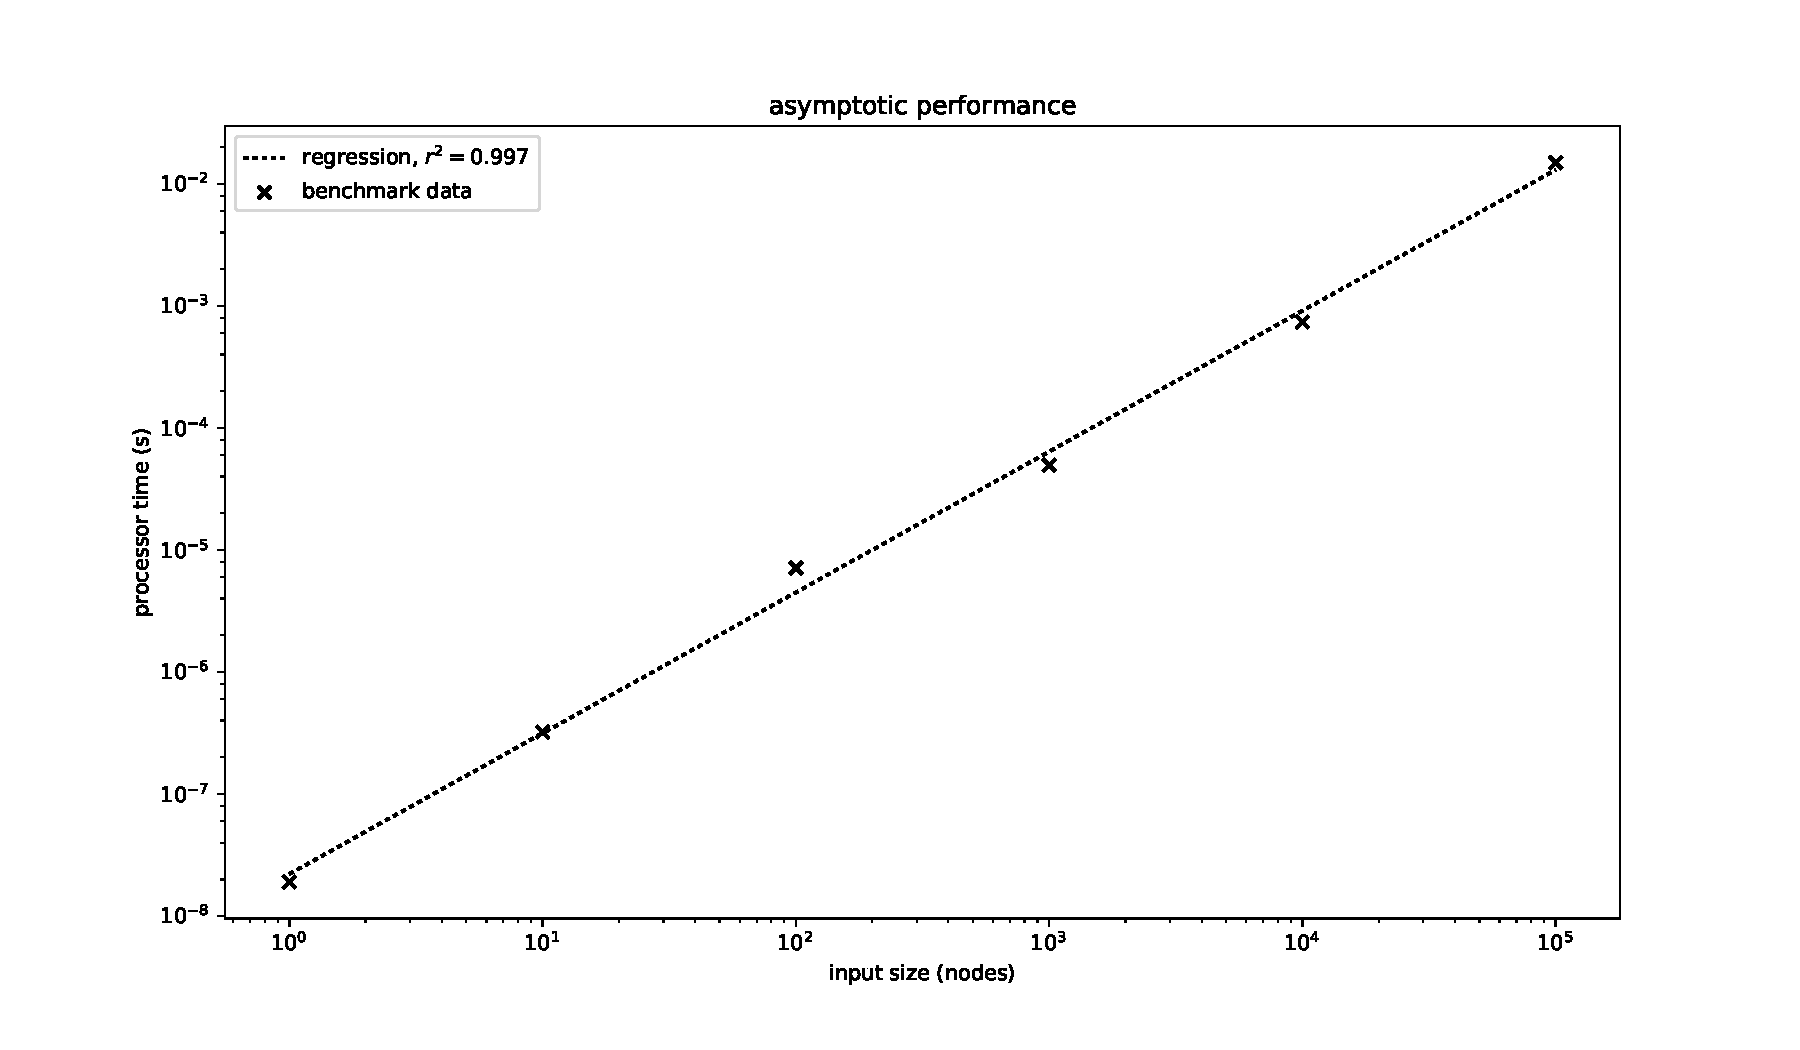
\includegraphics[width=\linewidth]{chapters/evaluation/plots/welltyped-map}
 \caption{asymptotic performance}
\end{subfigure}
\begin{subfigure}{.49\textwidth}
 \centering
 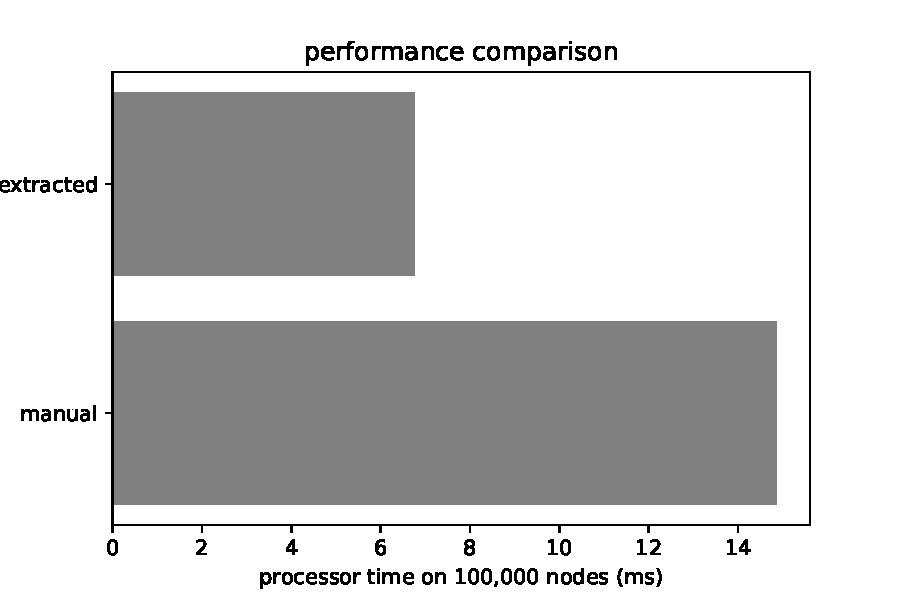
\includegraphics[width=\linewidth]{chapters/evaluation/plots/comparison}
 \caption{comparison against extracted code}
\end{subfigure}
\caption{plots showing the performance of the manual implementation}
\label{fig:results-map}
\end{figure}

\section{Comparison to Previous Work}
There have of course been other formalisations of typed \(\lambda\)-calculi.
Isabelle has its own implementation (in \texttt{\textasciitilde\textasciitilde/src/HOL/Proofs/Lambda/}), which I will use as a context in which to evaluate my project --- using another implementation written with different proof tools would confuse the issue, as different tools produce different approaches to play to their strengths and weaknesses.

Despite using the same tooling, the two implementations are still very different: Isabelle's implementation uses chained, tactic-style reasoning almost exclusively, introduces types separately to terms, and uses a nameless representation of bound variables, whereas my project uses explicit reasoning steps almost exclusively, attaches an explicit type to every binder, and uses a named representation, combined with the use of a quotient type to represent \(\alpha\)-equivalence.

\subsection{Chained Tactics vs. Isar}
Using only tactics does tend to make the proof shorter (as can be seen from the proof lengths for comparable lemmas in both implementations), but can also (albeit subjectively) decrease readability of the generated proof\cite{isar-phd}.
Another advantage of the Isar approach is ease of learning: if I could not get a tactic to show what I wanted, it was easier to break down the proof statement into smaller steps using Isar and invoke a prover on each than it was to learn what sequence of tactic applications would produce the desired result.

\subsection{Church- vs. Curry-style Types}
The Isabelle implementation actually formalises the untyped calculus, before adding simple types afterwards.
This approach allows for multiple type systems to be implemented on top of a base that deals only with untyped operations, a great improvement on my project, which would need to be re-written totally in order to add a significant change to the type system.

However, not adding explicit types to binders does produce a marked difference in what the theory shows: this is now Curry-style typing, where the question for type schemes given a term \(M\) is no longer the Church-style ``what is the type of \(M\)?'', but ``what is the set of possible types for \(M\)?''.
Of course, this is intentional --- but if a Church-style typing system is desired, then this approach is not possible.

One way to achieve this modularity in a Church-style context would be to parameterise the datatype for representing terms over all possible datatypes for representing types, as well as variables.
With this modification, adding a new type system would involve only defining a new datatype representing the new types, and building the new typing system around the term parameterised by these new types.

Even more generally, most of the work with binders and substitution could be done on an abstract notion of terms-with-names.
Consider defining \emph{abstract terms} \(\mathcal A\) to be either
\begin{enumerate}
\item a variable (bound or free) \(x\)
\item a pair \((\mathcal A, \mathcal A)\)
\item a binder \(x_C.\mathcal A\), binding a variable in an abstract term with some ``context'' \(C\)
\end{enumerate}
This is sufficient to define \(\alpha\)-equivalence, substitution and so forth.
Then define a bijection \(f\) between abstract terms and the concrete terms of the simply-typed calculus as follows:
\begin{align*}
f(x) &= x\\
f((M\ N)) &= (f(M), f(N))\\
f(\lambda (x : C). M) &= x_C.f(M)
\end{align*}
and the obvious definition of \(f^{-1}\).
All reasoning purely about operations involving names can now be done on the abstract terms, then added to the concrete terms by defining the concrete operation in terms of the abstract operation and \(f\).

By way of example, suppose the notion of substitution on abstract terms has been defined, and that we have proven Barendregt's substitution lemma --- that is, if \(x \neq y\) and \(x\) is not free in \(\mathcal L\), then
\[
\mathcal M[x ::= \mathcal N][y ::= \mathcal L] = \mathcal M[y ::= \mathcal L][x ::= \mathcal N[y ::= \mathcal L]]
\]
It can now be shown without proving the lemma again that this property holds for the concrete terms as well.
Define substitution on concrete terms (using a different notation for clarity) by reference to substitution on abstract terms, using \(f\) as follows:
\[
M[N/x] \equiv f^{-1}\wrap{f(M)[x ::= f(N)]}
\]
Then the lemma holds easily, since
\begin{align*}
M[N/x][L/y]
	&\equiv \wrap{f^{-1}\wrap{f(M)[x ::= f(N)]}}[y ::= L]\\
	&\equiv f^{-1}\wrap{f\wrap{f^{-1}\wrap{f(M)[x ::= f(N)]}}[y ::= f(L)]}\\
	&\equiv f^{-1}\wrap{f(M)[x ::= f(N)][y ::= f(L)]}\\
	&\equiv f^{-1}\wrap{f(M)[y ::= f(L)][x ::= f(N)[y ::= f(L)]]}\\
	&\equiv f^{-1}\wrap{f\wrap{M[L/y]}[x ::= f(N)[y ::= f(L)]]}\\
	&\equiv f^{-1}\wrap{f\wrap{M[L/y]}[x ::= f\wrap{N[L/y]}]}\\
	&\equiv M[L/y][N[L/y]/x]
\end{align*}

In this way a level of modularity and re-usability can be achieved, without sacrificing Church-style typing.
Had I thought of this earlier, I would undoubtedly have used this approach in my project!

\subsection{Approaches to Binders}
The treatment of binders is a difficult part of the formalisation of any system that uses them.
The authors of the \textsc{PoplMark} challenge\cite{poplmark} specifically mention this topic, and note that, of the solutions they have seen, there was no clear winner.

It can be seen from the extremely-small Isabelle implementation of deBruijn indices that a nameless representation (where \(\alpha\)-equivalence is simply equality) is much easier to formalise initially than the approach taken in my project --- no permutation lemmas, no \(\alpha\)-equivalence arguments, no quotient types...
However, the subsequent effort required to argue simple theorems such as the substitution lemma described above with deBruijn indices is significant.
Berghofer and Urban argue convincingly\cite{head-to-head} that a nominal representation has many advantages over indices, particularly in the context of the \textsc{PoplMark} challenge, once the initial infrastructure has been set up.

I think in this project the amount of effort required to implement a nominal representation was outweighed by the later benefits.
Additionally, the named representation is arguably more human-readable and presents less notational impedance than the nameless version, promoting later re-use.

\subsection{Nominal Implementation}
An important comparison to draw is that of a manual approach to a nominal implementation, with that of Nominal Isabelle.
I chose to perform things manually, as neither Nominal Isabelle, nor its successor Nominal 2 support code generation at the time of writing, and code generation was a required part of the project.

Unfortunately, this led to a lot of effort, that while educational, could have been avoided with use of the automation provided by Nominal Isabelle.
I had to manually implement:
\begin{itemize}
\item
A theory of permutations.
\item
(strong) Induction principles for \(\alpha\)-equivalent terms.
\item
A quotient type.
\item
Inequality rules for these terms, such as \(\forall A, B.\ (A, B) \neq \unit\) --- these are particularly unfortunate as the number of lemmas required grow quadratically with the number of different varieties of term.
\item
Structural equality rules, such as \(\forall A, B.\wrap{\pi_1(A) = \pi_1(B) \implies A = B}\).
\item
Proofs showing that functions on pre-quotient terms can also be functions on \(\alpha\)-equivalence classes, like the type inference function, then lifting them over the quotient.
This property is not true in general (consider the function that returns the bound variables of a term), but Nominal Isabelle provides a couple of ways to define functions which generate a proof obligation to show this property\cite{fresh-fun}.
\end{itemize}
